\chapter{Grundlagen}
Im folgenden Abschnitt sollen die Grundlagen, die für diese Arbeit relevant sind näher erläutert werden.

\section{Raspberry Pi} \chapterauthor{Dominic Steinhauser}
Der Einplatinencomputer ist ein zentrales Konstrukt, um den perfekten Raum zu verwirklichen. Durch das Anschließen von Sensoren können Bedingungen über das regelbasierte System für den perfekten Raum definiert und überwacht werden. Außerdem lässt sich durch den Anschluss eines Kameramoduls der Raum auf Bewegung prüfen. Das Ziel beim Betreiben eines solches Computers in einem Raum ist, einer Person dabei zu helfen seine Umgebung auf perfekte Eigenschaften zu kontrollieren und überwachen, sodass diese sich in ihrer Umgebung stets wohlfühlt. 
\\Außerdem wird der Raspberry Pi als Webserver eingesetzt, um Daten verschiedenen Applikationen bereitzustellen. 

\subsection{Webserver}
Um Informationen über das lokale Netzwerk oder im Internet zu teilen ist es notwendig, dass ein Webserver auf dem Raspberry Pi ausgeführt wird\cite{t3n:t3n}. Dieser bildet einen Einstiegspunkt, um Daten anderen Anwendungen bereitzustellen. Außerdem müssen die Sensoren integriert bzw. anfallende Daten in einer Datenbank gespeichert werden können. Deshalb ergaben sich bei der Auswahl des Webserver folgende Kriterien:
\begin{itemize}
	\item \textbf{Eventbasierte Engine}: Anfragen von Anwendungen sollen bei Bedarf bearbeitet werden
	\item \textbf{Erweiterbarkeit}: Hinzufügen neuer serverseitiger Schnittstellen muss gewährleistet sein
	\item \textbf{Integration/ Zugriff auf Sensoren}: Hinzufügen eines neuen Sensor sollte möglichst einfach sein
\end{itemize} 
Diese Anforderungen an einen Webserver decken Node.js, Apache und Node-RED ab. Wobei letzteres über die einfache und schnelle Erstellung von Services über eine Benutzerschnittstelle am meisten zusagt und am wenigsten Einarbeitungszeit voraussetzt.
\subsubsection{Node-RED}
Node Red wurde von IBM im Jahre 2013 entwickelt und steht als Open-Source Projekt zur Verfügung\cite{nodeRed:nodeRedAbout}.\\
Mithilfe von Node Red, das auf Node.js basiert, können Datenflüsse bzw. Flows über eine Benutzerschnittstelle im Browser zum Ausführen vom serverseitigen Aufgaben angelegt werden. Dabei werden verschiedene Knoten, auch Nodes genannt, miteinander verknüpft. \autoref{img:bspFlow} zeigt beispielhaft ein Flow auf, der aus den Knoten \acf{HTTP} Input, einer Funktion, und dem \ac{HTTP} besteht. Jeder Knoten stellt somit eine spezifische Funktionalität bereit. Der \ac{HTTP} Input Node, definiert den Eintrittspunkt bzw. den relativen Pfad, an den \ac{HTTP} Anfragen vom Client gesendet werden. Als Ergebnis liefert der angelegte Flow eine Antwort auf die \ac{HTTP} Anfrage zurück. Die Anwendungslogik kann durch Javascript in dem sogenannten Function Node in den Datenfluss integriert werden . Die miteinander verbundenen Knoten reichen sich außerdem Daten oder Informationen über \ac{JSON}-Objekte weiter.
\\Schließlich können die einzeln erstellten Flows einfach innerhalb der Laufzeitumgebung deployed und ausgeführt werden. \\Durch eine große Community werden neben den standardmäßigen Knoten auch neue Knoten bereitgestellt, die den Funktionsumfang von Node Red nochmals deutlich erweitern\cite{nodeRed:nodeRed}.
\begin{figure}[H]
	\centering	
	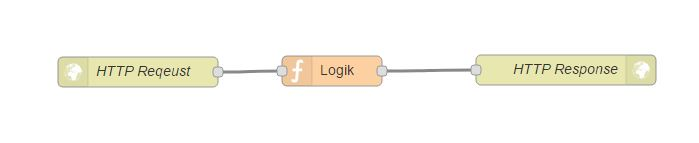
\includegraphics[scale=0.8]{images/bspFlow}
	\caption{Beispiel eines Node-RED Flows}
	\label{img:bspFlow}
\end{figure}




\section{Datenbank}\chapterauthor{Dominic Steinhauser}
Durch die Anbindung von Sensoren werden ständig neue Daten generiert. Damit diese Daten für spätere Zwecke genutzt werden können, wie beispielsweise für die Analyse oder Erzeugen von Vorhersagen, ist es hilfreich diese zentral an einem Ort in einer Datenbanklösung abzuspeichern.
\\NoSQL Datenbanken benötigen kein vordefiniertes Schema, um Daten abzuspeichern. Somit ist es nicht notwendig zu wissen welche Art von Daten bzw. deren Datentypen gespeichert werden sollen. Der Vorteil ergibt sich dabei, dass zusammengehörende Daten gemeinsam an einem Ort abgespeichert werden. Der Datentyp jedes einzelnen Eintrags kann dabei von Eintrag zu Eintrag variieren. Deshalb sind für diese Datenbanklösungen Strukturänderungen im Datenformat problemlos. Sollte die Datenbank sehr groß werden und auf mehreren Servern laufen, so lassen sich diese einfach skalieren\cite{noSQL:noSQL}.
\\Außerdem gibt es noch die Möglichkeit Daten innerhalb von relationalen Datenbanken abzuspeichern. Dabei muss zuerst ein Datenbankschema definiert werden. Hierbei ist also die abzuspeichernde Datenstruktur im Voraus bereits definiert und kann im Vergleich zu NoSQL-Datenbanken nicht einfach im Betrieb angepasst werden. Die Ablagestruktur in Tabellen sollte sich dabei am natürlichen Vorkommen der Daten (Bsp.: Name, Vorname, Straße, PLZ, Ort)  orientieren. Jede Zeile einer Relation steht für ein Tupel, das eine strikte Ordnung der Attribute voraussetzt\cite{codd:Codd}. Folglich muss beim Einfügen auf die Struktur geachtet werden.
\\Da angenommen werden kann, dass die angeschlossenen Sensoren durchgängig gleiche Datenformate an den Raspberry Pi übermitteln und sich somit die Struktur nicht ändert, wird für den folgenden Verlauf der Arbeit ein relationales Datenmodell als Grundlage definiert.
\\\\Da der Raspberry Pi vergleichsweise wenig Hardwareressourcen besitzt, muss darauf geachtet werden, dass die Datenbank ressourcenschonend arbeitet. Die Datenbank soll lokal vom Raspberry betrieben und muss nur wenige bis keine von extern über das Netzwerk kommenden Datenbankeinträge erstellen.\\Im Vergleich zwischen der SQLite und der MySql Datenbanklösung fällt die Entscheidung auf SQLite. Diese Lösung bringt für das Abspeichern von Daten alle notwendigen Funktionalitäten mit, wie Datenbankzugriff mit \acf{SQL} oder die vorhandenen Datentypen \cite{sqlite:sqlite2}, ohne jedoch wie MySql  viele Features anzubieten, die für diese Arbeit nicht gebraucht werden. Beispiel hierfür wäre ein eigener Datenbankserver, mit dem Anwendungen über einen Prozess kommunizieren müssen. Außerdem werden Datenbankeinträge nur vom einem Raspberry Pi erzeugt, der dann Embeded System angesehen werden kann und somit die SQLite Datenbank ausreicht. Die Größe der Datenmenge wird nicht dazu führen, dass schnell eine mehrere Gigabyte große Datenbank entsteht, die dann skaliert  und dafür eine andere Lösung als SQLite eingesetzt werden muss.\cite{sqlite:sqlite}


\section{Regelbasiertes System} \chapterauthor{Louisa Pabst}
Im heutigen Alltag werden kontinuierlich Daten erfasst, um auf dessen Basis Informationen zu erhalten. Daten werden aus unterschiedlichen Gründen gesammelt, meist steht jedoch hinter der Datensammlung der Wunsch einen Mehrwert aus den Daten zu schaffen. Um Daten nutzen zu können, müssen diese kanalisiert, strukturiert und archiviert werden \cite{managermagazin:datensammlung}. Regelbasierte Systeme \acs{RBS}, die eine Sonderform eines Expertensystems bilden \cite{ieee:ruleBasedSystemAndNetworks}, werden für die Datenstrukturierung eingesetzt. Ursrprünglich stellten diese Systeme ledigliche mithilfe von menschlichem Expertenwissen codierte Problemlösungen dar \cite{Hayes-Roth:1985:RS:4284.4286}. Im Laufe der Zeit hat sich diese Definition erweitert. Neben Regeln, die von einem Experten gesetzt werden, stellen regelbasierte Systeme auch Regeln auf, die auf Basis historischer Datensätze erstellt werden. Aus diesem Grund wird bei der Erstellung eines solchen Systems zwischen einem experten- und einem datenbasierten Design unterschieden. Gerade im Zuge der stark ansteigenden Datenmengen findet man regelbasierte Systeme mit einem Daten basiertem Design vergleichsweise häufiger im Einsatz \cite{ieee:ruleBasedSystemAndNetworks}.\\
Die problemlösenden Methoden werden in einem \ac{RBS} durch Situation-Aktion Regeln abgebildet. Um sinnvolle Lösungen zu Problemstellungen zu erlangen, sollten die folgenden fünf Punkte beim Aufstellen von Regeln beachtet werden.\\
Das Wissen sollte in Wenn-Dann-Regeln aufgestellt werden. Die Bedingung für die Ausführung der Regel wird im ersten Teil der Regel definiert, dem Wenn-Teil. Dabei können mehrere Konditionen aneinander geknüpft werden. Im zweiten Teil der Regel, dem Dann-Teil, wird die Aktion beschrieben, die nach der Erfüllung der Kondition ausgeführt wird. Es kann davon ausgegangen werden, dass wenn die Kondition erfüllt ist, auch die Aktion erfüllt ist. Eine \ac{RBS} kann aus diesem Grund als Interpreter von Wenn-Dann-Regeln gesehen werden\cite{oracle:JREAPI}.\\
Neben der Darstellung einer Regel durch die Wenn-Dann Form, können Regeln auch durch Entscheidungstabellen abgebildet werden \cite{HSAugsburg:RuleEngine}. Entscheidungstabellen verknüpfen Aktionen mit Bedingungen \cite{itwissen:entscheidungstabelle}. Der Unterschied zu den zuvor beschriebenen Wenn-Dann-Regeln ist die formale Aufstellung der Regeln in Form von einer Tabellenstruktur.\\
Als nächsten Punkt, den man beim Aufstellen von Regeln beachten soll, ist die Steigerung der Kompetenz des \ac{RBS} proportional zur Wissenserweiterung. Wenn diese Steigerungen nicht proportional zueinander verlaufen, wird das \ac{RBS} auf lange Sicht nicht den gewünschten Mehrwert mit sich bringen.\\
Des Weiteren sollte das \ac{RBS} durch Kombination von Regeln auch komplexere Problemstellungen lösen. Dabei werden die Ergebnisse der Regelausführung sinnvoll kombiniert. Um Probleme bestmöglich lösen zu können, sollten \ac{RBS} die optimale Reihenfolge von Regeln bestimmen und anschließend ausführen. Die nach Durchführung der Regel erhaltene Lösung zur Problemstellung sollte vom System anschließend in natürliche Sprache oder in Aktionen, die für den Menschen verständlich sind, übersetzt werden.\\
Genutztes Wissen innerhalb eines \ac{RBS} wird als problemlösendes Wissen bezeichnet und besteht aus verschiedenen Formen von Informationen. So können Informationen durch Beobachtungen gesammelt werden, sowie durch Abstrahierung, Generalisierung oder Kategorisierung von gegebenen Daten. Neben reinen Daten werden Verknüpfungen von Daten sowie Stratgien zur Datengewinnung als relevante Informationen angesehen \cite{Hayes-Roth:1985:RS:4284.4286}.\\
Bei der Erstellung eines \ac{RBS} muss jedoch beachtet werden, dass ein geeignetes System stetig angepasst und verbessert werden muss. Vor allem müssen Lösungen durch hinzukommendes Wissen optimiert werden können.\cite{Hayes-Roth:1985:RS:4284.4286}.



